\section{Results}
\label{sec:results}

\begin{figure*}[t]
\centering
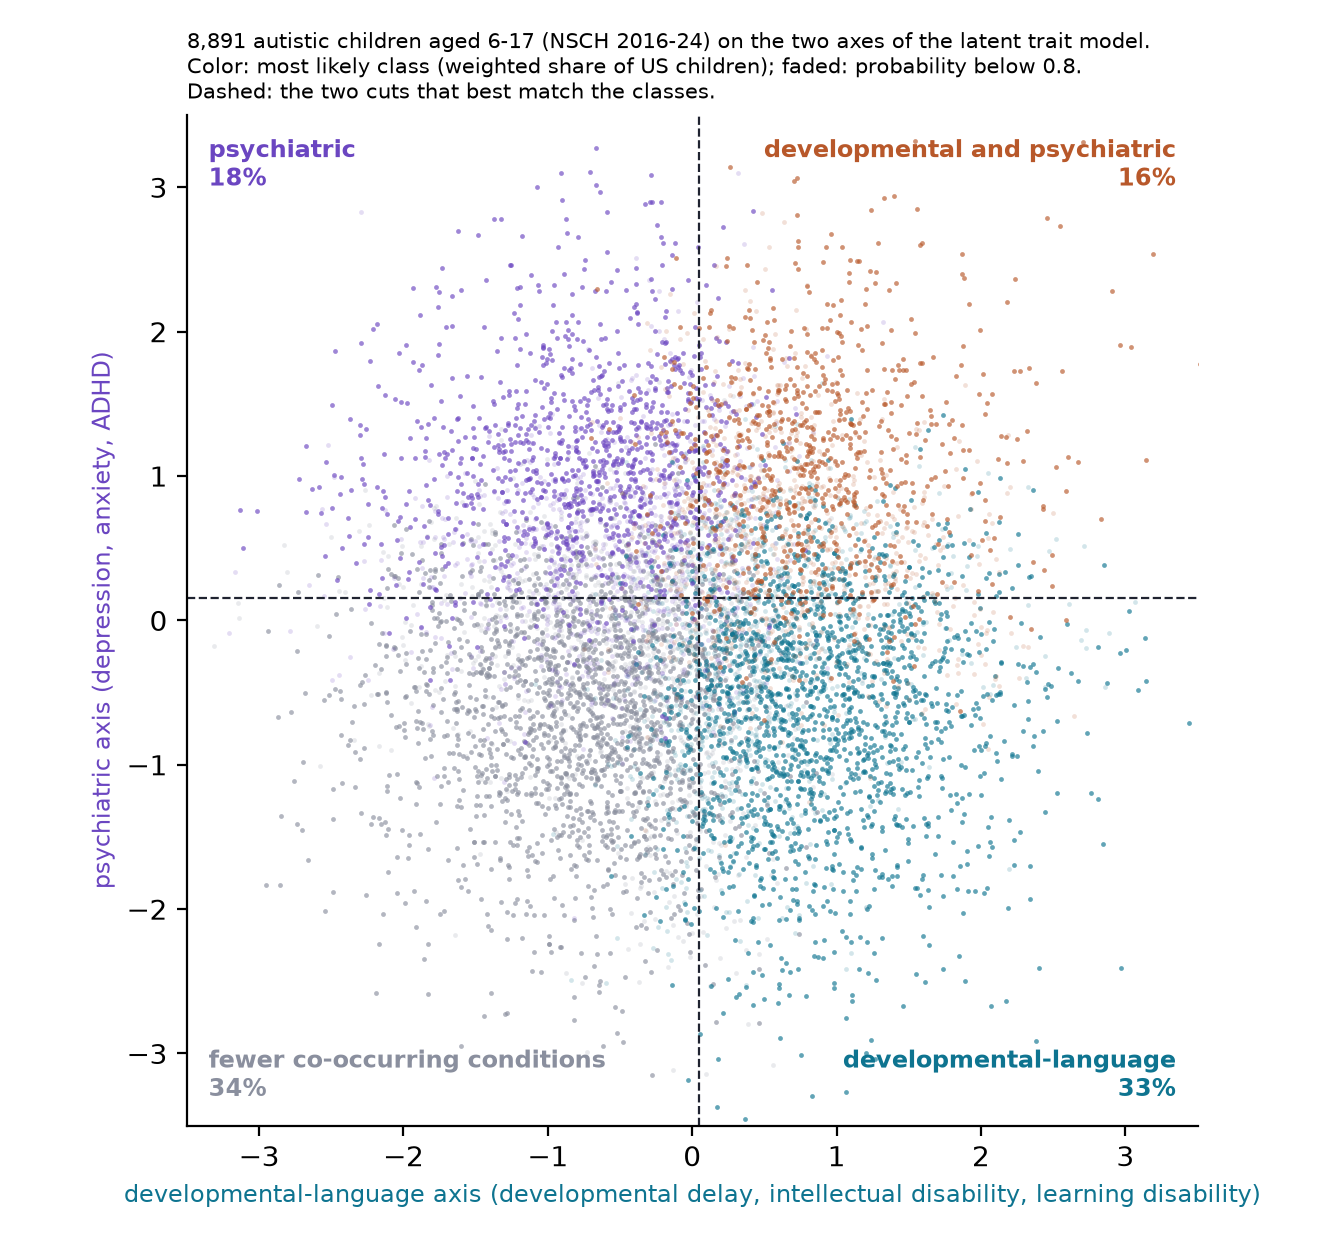
\includegraphics[width=0.62\textwidth]{figure1_map.png}
\caption{The 8,891 children placed on the two axes of the latent trait model (one draw from each child's posterior). Color is the most likely of the four latent classes; children whose largest class probability is below 0.8 are faded. Dashed lines are the two cuts on the axes that best reproduce the classes (ARI 0.80). The corner labels give each class's weighted share of US autistic children aged 6 to 17. The children form one cloud, and the classes are its quadrants.}
\label{fig:map}
\end{figure*}

\subsection{Two axes}
\label{sec:axes}
Figure~\ref{fig:map} shows the result the rest of the section builds toward. The two-dimensional latent trait model separates the 18 conditions into two sets (Figure~\ref{fig:loadings}). A developmental-language axis carries developmental delay (slope 3.97), intellectual disability (3.14), learning disability (2.51), Down syndrome (2.19) and speech or language disorder (2.03), with cerebral palsy and epilepsy more weakly. A psychiatric axis carries depression (3.63), anxiety (2.51), headaches (1.13), ADHD (0.89) and Tourette syndrome (0.87). Behavior problems load on both (0.68 and 0.73). Bootstrap standard errors for the slopes are 0.03 to 0.28, and the same two axes appear when the model is fit separately to ages 6 to 11 and 12 to 17 (congruence 0.98 or higher). The psychiatric position rises with age (correlation 0.26), which matches when anxiety and depression are usually diagnosed, and the developmental position falls slightly ($-0.11$).

The four latent classes of Section~\ref{sec:profiles} are the four combinations of high and low on these axes. Two cuts on the axes, placed at the class means, reproduce the class assignments at ARI 0.80. The children do not form four separate clumps: they form one cloud, and the children whose class is uncertain lie along the cuts.

\begin{figure}[t]
\centering
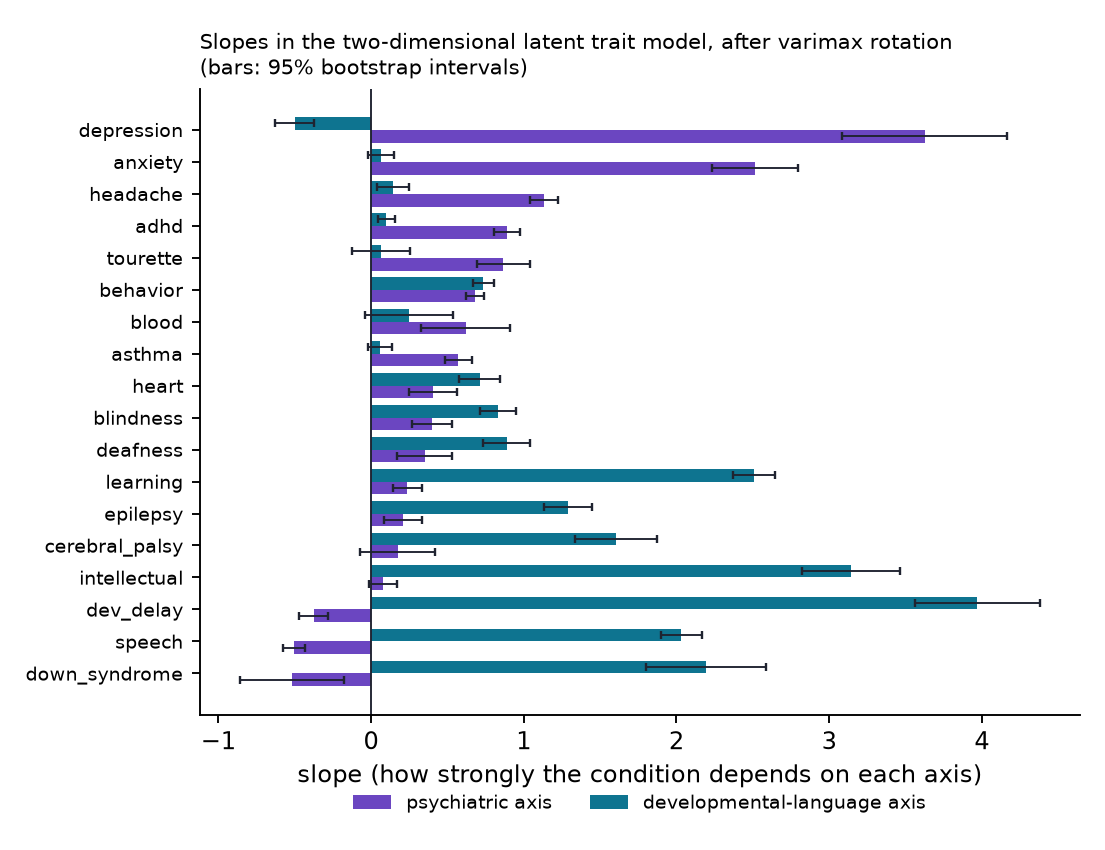
\includegraphics[width=\columnwidth]{loadings.png}
\caption{Slopes of the two-dimensional latent trait model, with 95\% intervals from 50 bootstrap refits. Each condition loads mainly on one axis; behavior problems load on both.}
\label{fig:loadings}
\end{figure}

\subsection{How many classes}
\label{sec:howmany}
BIC fell at every $K$ from 1 to 8, while the shuffled baseline rose throughout, so there is structure, but no $K$ is selected: the drops shrink from 8,224 ($K=1$ to 2) to 6 ($K=7$ to 8), and every class added after $K=5$ holds under 3\% of children. Held-out likelihood also improves through $K=8$ (Table~\ref{tab:models}). By the stability rule, the least stable class has mean Jaccard 0.91 at $K=4$, 0.63 at $K=5$, 0.55 at $K=6$, 0.64 at $K=7$ and 0.58 at $K=8$, so the rule gives $K=4$. The choice does not depend on the threshold or the number of resamples: at thresholds of 0.7, 0.75 and 0.8, with 50, 100 or 200 resamples, $K=4$ is the only $K$ that passes, and it is also the most stable $K$ tested.

The calibration limits what this means. On data simulated from the two-dimensional model, which has no classes, every class is stable through $K=5$ (least stable 0.84 at $K=4$ and 0.88 at $K=5$) and stability breaks only at $K=6$. A smooth cloud can be cut into four or five pieces that come back in every resample, so the rule finds the finest division that reproduces, not the number of groups. On data simulated from the $K=5$ class model all five classes are stable (0.92 or more, including an 8\% class), so the real fifth class does not fail for being small.

\begin{table}[t]
\centering
\caption{Classes against dimensions. BIC on 2016 to 2024; held-out log-likelihood as the difference from the three-dimensional model, the best one that is not degenerate (standard error). $D=4$ ends on the slope bound and is not interpreted.}
\label{tab:models}
\small
\setlength{\tabcolsep}{4pt}
\begin{tabular}{lrrrr}
\toprule
Model & Param. & BIC & 2022--24 & 2025 \\
\midrule
Classes, $K=4$ & 75 & 106,427 & $-286$ (32) & $-106$ (16) \\
Classes, $K=5$ & 94 & 105,959 & $-182$ (25) & $-64$ (13) \\
Classes, $K=8$ & 151 & 105,655 & $-60$ (22) & $-23$ (11) \\
Trait, $D=1$ & 36 & 109,198 & $-1063$ (50) & $-374$ (29) \\
Trait, $D=2$ & 53 & 105,291 & $-57$ (14) & $-26$ (8) \\
Trait, $D=3$ & 69 & 105,095 & 0 & 0 \\
Trait, $D=4$ & 84 & (104,909) & ($+54$) & ($+14$) \\
\bottomrule
\end{tabular}
\end{table}

\subsection{The four profiles}
\label{sec:profiles}

\begin{figure*}[t]
\centering
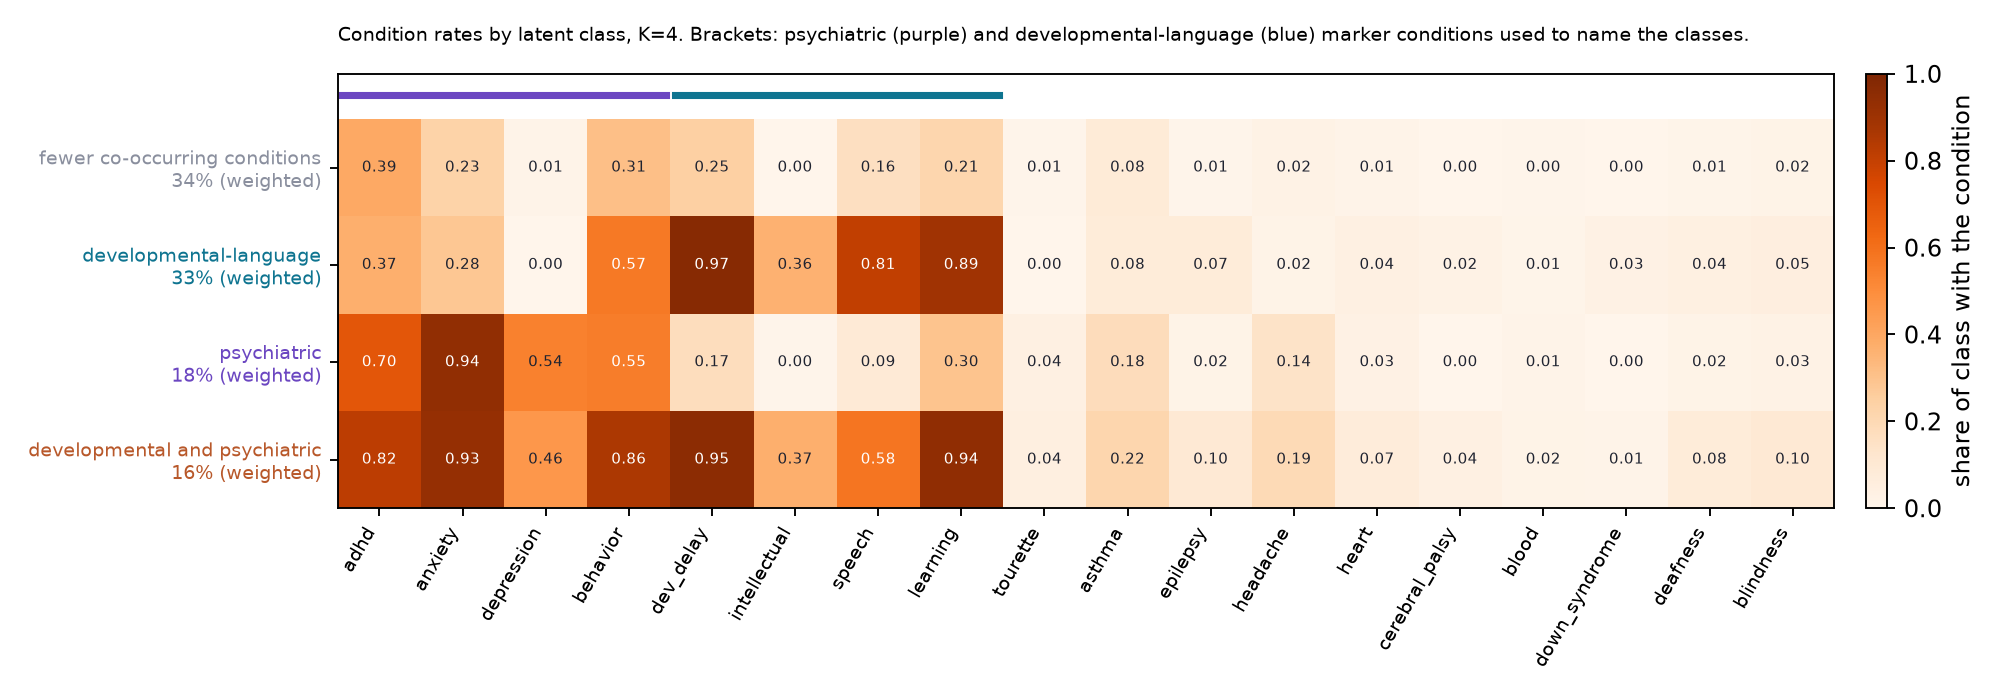
\includegraphics[width=\textwidth]{classes.png}
\caption{Condition rates in the four latent classes ($K=4$), with weighted shares of US autistic children aged 6 to 17. Bars above mark the psychiatric (purple) and developmental-language (blue) conditions used to name the classes.}
\label{fig:classes}
\end{figure*}

\begin{stub}{Haley, about 0.4 column}
Walk through Figure~\ref{fig:classes}. Weighted shares with 95\% intervals (\texttt{results\_k4/shares.csv}): fewer co-occurring conditions 34\% (32 to 36), developmental-language 33\% (31 to 35), psychiatric 18\% (16 to 19), developmental and psychiatric 16\% (14 to 17). Defining rates: developmental-language has developmental delay 0.97, learning 0.89, speech 0.81, intellectual 0.36; psychiatric has anxiety 0.94, ADHD 0.70, depression 0.54; both has ADHD 0.82, anxiety 0.93, behavior 0.86, delay 0.95, learning 0.94; fewer has nothing above 0.39 (ADHD). Medical conditions are low everywhere and highest in the ``both'' class. Age and sex by class (\texttt{results\_k4/demographics.csv}). Assignment certainty: relative entropy 0.72; a quarter of children have no class above 0.7. Shares by year (\texttt{reports/figures/results/shares\_by\_year.png}) stay within their intervals; ``both'' drifts from 19\% in 2016 to 14\% in 2024; 2025 shares within 3.2 points of the pooled shares.
\end{stub}

\subsection{What replicates, and what that shows}
\label{sec:replication}

\begin{figure}[t]
\centering
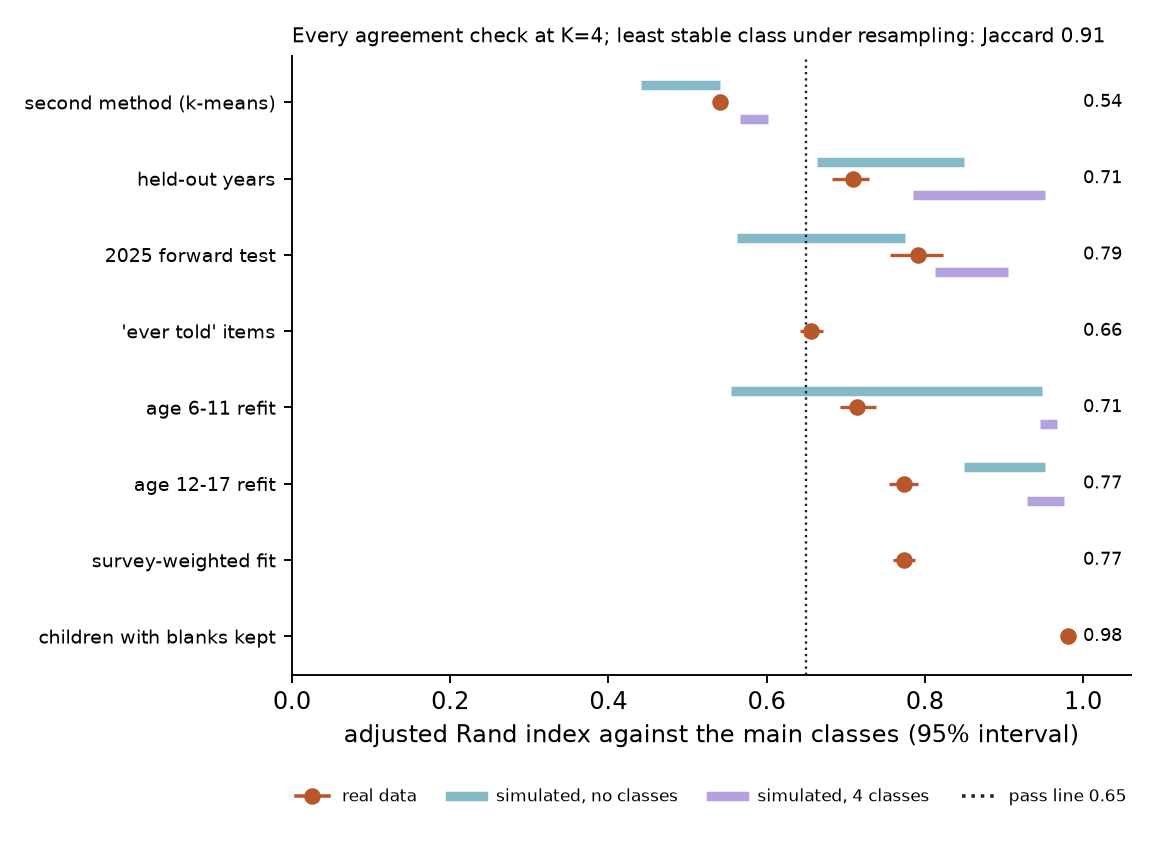
\includegraphics[width=\columnwidth]{checks_k4.png}
\caption{Every agreement check at $K=4$ (dots, with 95\% intervals from resampling children), beside the range the same check gives on five datasets simulated from the two-dimensional model with no classes (teal) and five from the four-class model (lilac). Dotted line: the 0.65 pass line.}
\label{fig:checks}
\end{figure}

Table~\ref{tab:checks} and Figure~\ref{fig:checks} give every check at $K=4$. The classes pass the independent replications: fit separately on 2016 to 2021 and on 2022 to 2024, the two models label the later children at ARI 0.71 (0.68 to 0.73), and the frozen model and a fresh fit agree on the 2025 children at 0.79 (0.76 to 0.82). They pass within each age band (0.71 and 0.77) and under resampling (every class's mean Jaccard 0.91 to 0.93). The ``ever told'' items give 0.66 (0.64 to 0.67), on the line. The survey-weighted fit agrees at 0.77, refits from five other seeds at 1.00, and the refit that keeps the 819 children with blank answers at 0.98, with class sizes within half a point.

The second method fails. $k$-means agrees with the classes at 0.54, and across five seeds its best solutions differ in total distance by about 0.01\% and agree with the classes at 0.52 to 0.58. The disagreement is at the borders: among the 52\% of children the class model places with probability 0.9 or more, $k$-means agrees at 0.93. The proposal's average-linkage hierarchical clustering on Jaccard distance failed outright, putting 94\% of children in one cluster at every $K$ from 4 to 6 (ARI 0.00). With 18 yes/no items, thousands of children sit at small distances from one another, average linkage chains through them, and the 517 children with no conditions form a separate point. Complete linkage, prevalence-weighted Jaccard and spectral clustering do no better (0.08 or less), and Ward linkage reaches 0.34.

\begin{table}[t]
\centering
\caption{Checks at $K=4$: real ARI with its 95\% interval, beside the range over five datasets simulated from the two-dimensional model (no classes) and five from the four-class model. Pass line 0.65.}
\label{tab:checks}
\small
\setlength{\tabcolsep}{3pt}
\begin{tabular}{lccc}
\toprule
Check & Real & Continuum & 4 classes \\
\midrule
Held-out years & 0.71 (0.68--0.73) & 0.66--0.85 & 0.78--0.95 \\
2025 forward test & 0.79 (0.76--0.82) & 0.56--0.78 & 0.81--0.91 \\
Age 6--11 & 0.71 (0.69--0.74) & 0.56--0.95 & 0.95--0.97 \\
Age 12--17 & 0.77 (0.76--0.79) & 0.85--0.95 & 0.93--0.98 \\
$k$-means & 0.54 & 0.44--0.54 & 0.57--0.60 \\
``Ever told'' items & 0.66 (0.64--0.67) & & \\
Weighted fit & 0.77 (0.76--0.79) & & \\
Blanks kept & 0.98 (0.98--0.99) & & \\
\midrule
Bootstrap Jaccard & 0.91 (least) & 0.84 & 0.92$^{a}$ \\
\bottomrule
\end{tabular}
\\[2pt]{\footnotesize $^{a}$ Least stable class in the five-class simulation at $K=5$.}
\end{table}

The calibration changes how these passes read. A four-way cut of the simulated continuum, which has no groups in it, reproduces across held-out years at 0.66 to 0.85, in a fresh 2025-sized sample at 0.56 to 0.78, within age bands at 0.56 to 0.95 and 0.85 to 0.95, and against $k$-means at 0.44 to 0.54. Data with four real classes reproduce better on every check: 0.78 to 0.95 across years, 0.81 to 0.91 in 2025, 0.93 to 0.98 within age bands and 0.57 to 0.60 against $k$-means. The real values sit inside the continuum's range for held-out years, the younger band and $k$-means, just above it for 2025 (0.79 against 0.78) and below it for the older band, and below the four-class range on every check. So the partition is reproducible, as a partition of a continuum also is, and the replication checks cannot by themselves say that its pieces are groups. On every check the real data replicate the way a continuum does.

\subsection{Classes or dimensions}
\label{sec:classes-or-dimensions}
The continuous model describes the data better (Table~\ref{tab:models}, Figure~\ref{fig:fit}). With 53 parameters, $D=2$ has a lower BIC than any class model, including $K=8$ with 151. On held-out years it predicts as well as eight classes: measured from $D=3$, $D=2$ trails by 57 log-likelihood units (standard error 14) on 2022 to 2024 and by 26 (8) on 2025, and $K=8$ by 60 (22) and 23 (11), while $K=4$ trails by 286 and 106. $D=4$ is degenerate: one dimension collapses onto ADHD and its slope runs to the bound.

\begin{figure}[t]
\centering
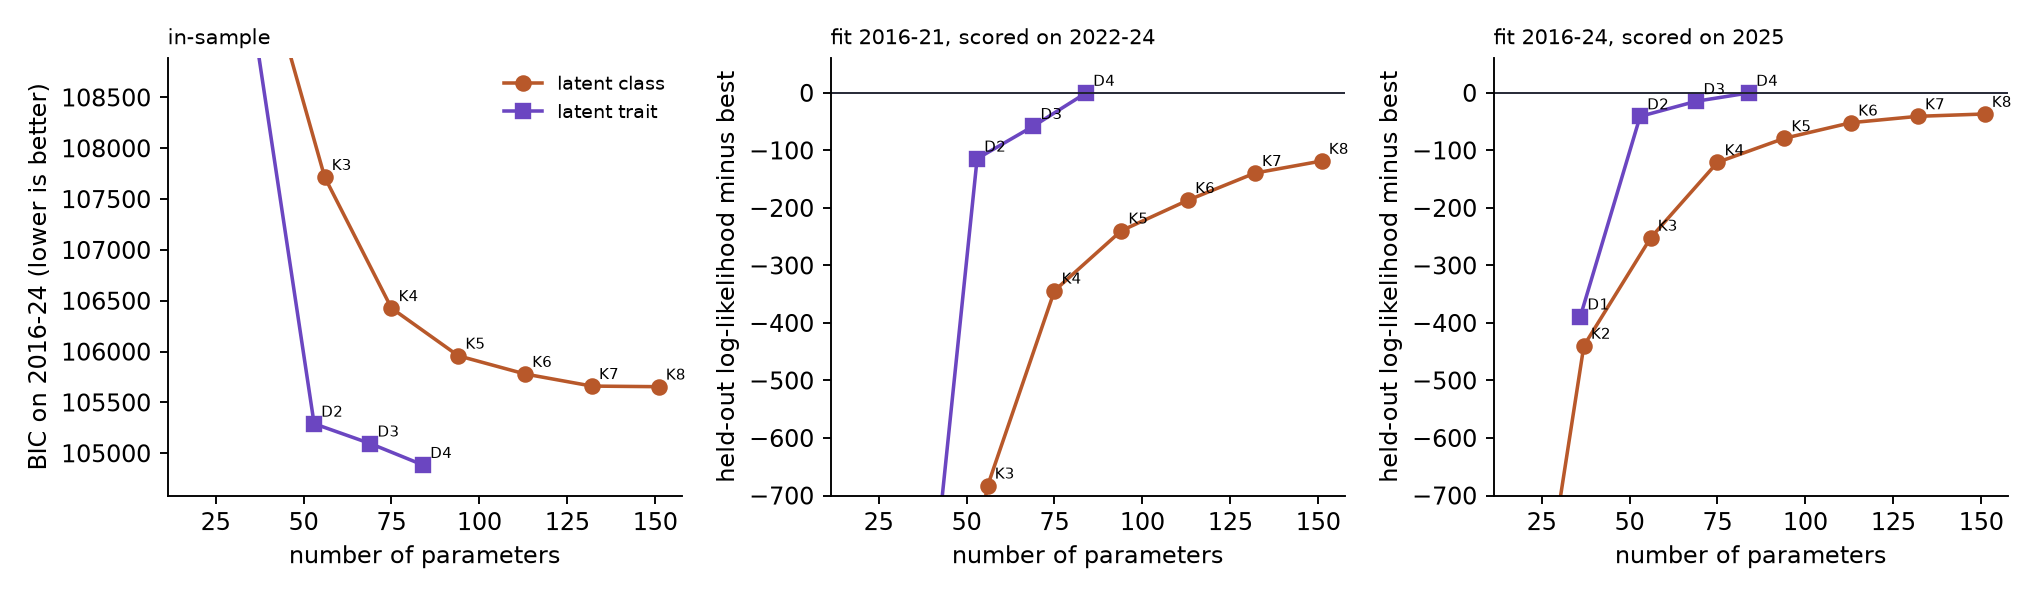
\includegraphics[width=\columnwidth]{model_fit.png}
\caption{In-sample BIC and held-out log-likelihood for latent class models ($K=1$ to 8) and latent trait models ($D=1$ to 4). $D=4$ (hollow) ends on the slope bound.}
\label{fig:fit}
\end{figure}

Three further results point the same way. Data simulated from the fitted $D=2$ model give a class BIC curve that keeps falling through $K=6$, as the real one does, while data simulated from four classes give a curve that turns up at $K=4$, so this comparison can tell the two apart and the real data behave like the continuum \citep{bauer2004}. The model with three dimensions adds a medical-sensory axis (cerebral palsy, deafness, blindness, Down syndrome, epilepsy, headaches) and cuts the pairs of conditions with poor fit from 49 to 36 of 153; pairs such as deafness with blindness and epilepsy with cerebral palsy are among those the $K=4$ and $D=2$ models fit worst. And the estimated distribution of positions is not a bell curve: it improves on the normal by 94 log-likelihood units, against 16 to 22 for data simulated from the continuum and 180 to 199 for data from four classes. The real children are lumpier than a smooth cloud and about half as lumpy as four separate groups, which is the pattern a factor mixture model would describe.

\subsection{Severity}
\label{sec:severity}

\begin{figure}[t]
\centering
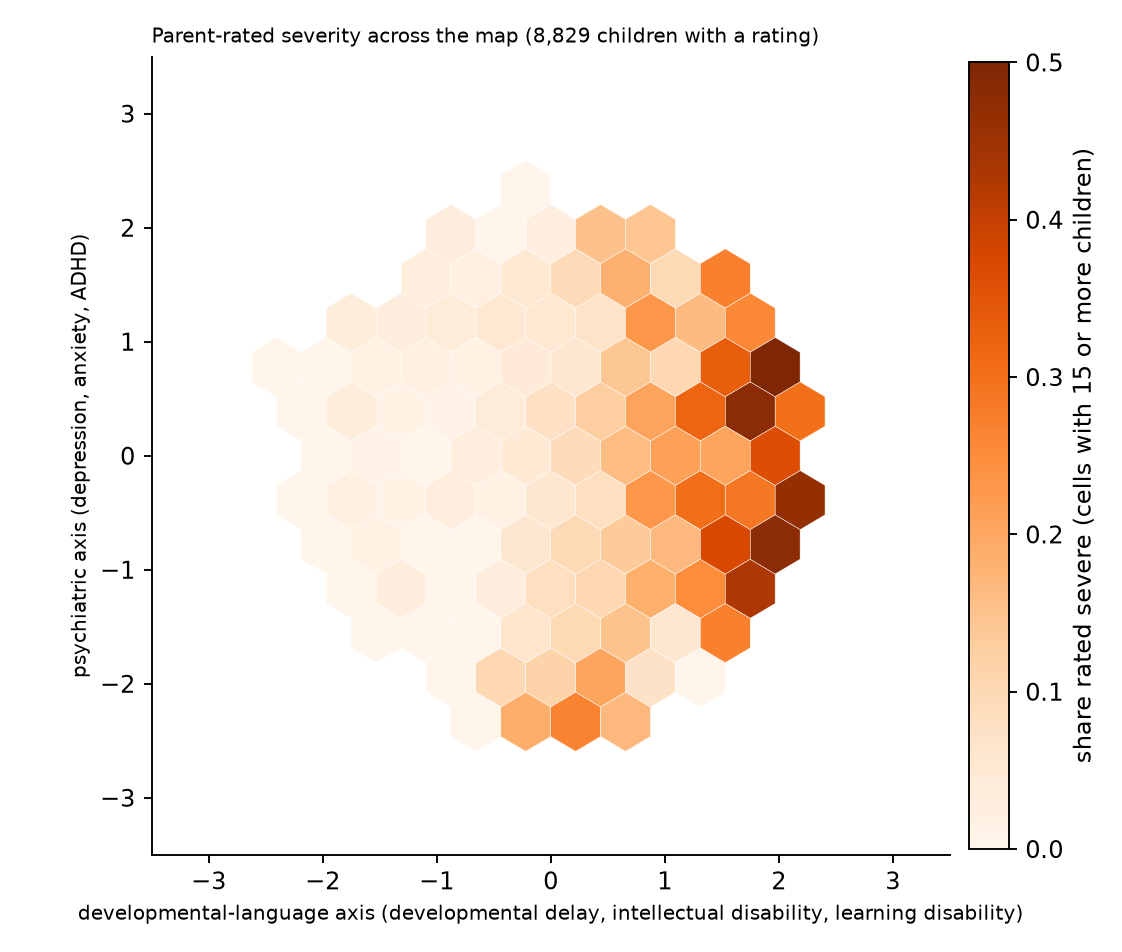
\includegraphics[width=\columnwidth]{severity_map.png}
\caption{Share of children rated severe across the map of Figure~\ref{fig:map} (hexagons with 15 or more children). Severity rises along the developmental-language axis and does not jump at the class borders.}
\label{fig:severity}
\end{figure}

\begin{stub}{Haley, about 0.4 column}
Severity by class (\texttt{results\_k4/severity\_by\_class.csv}, \texttt{reports/figures/results/severity\_by\_class.png}): rated severe 21\% in developmental-language and in both, 2\% in fewer, 4\% in psychiatric. Figure~\ref{fig:severity}: rises along the developmental axis, no jump at the borders. The planned test (\texttt{results\_k4/count\_vs\_class.csv}): count plus class beats count on BIC (14,447 against 14,873) and log-loss (0.815 against 0.840); class alone does not (BIC 14,996; log-loss 0.846). So the classes pass on one reading of the pre-fit sentence and fail on the other. Comparators: class probabilities 14,622; the two factor scores alone 14,262 with 6 parameters, better than count plus class; scores plus class 14,243; all 18 flags 14,159. Severity and flags come from the same parent in one interview, so part of any association is shared reporting style; model comparisons are less affected than any single association.
\end{stub}

\subsection{Five classes}
\label{sec:k5}
\begin{stub}{Haley, about 0.25 column}
$K=5$ (\texttt{results\_k5/}): adds a class with intellectual disability, speech and developmental delay near 1 and the highest rates of epilepsy, cerebral palsy, Down syndrome, deafness and blindness; 9\% weighted, 45\% rated severe. It appears in every resample but its membership does not hold (Jaccard 0.63); held-out years fail (ARI 0.635, 0.62 to 0.65); weighted fit disagrees (0.59); 2025 0.78 and age bands 0.79 and 0.85 pass. Same signal as the third (medical-sensory) dimension. Corresponds to the ``broadly affected'' groups of \citet{vargason2019} (24\%) and \citet{litman2025} (10\%). Past $K=5$ the replication and 2025 tests fail too (\texttt{reports/tables/checks\_by\_k.csv}).
\end{stub}
